\documentclass[tikz,border=2pt]{standalone}
\usepackage{tikz}
\usepackage{lmodern}
\usetikzlibrary{calc,decorations.pathreplacing}

% Visual conventions follow the existing MRNC TikZ pictures: ordinary
% components use TikZ's normal 0.4pt stroke, with compact TeX labels.
\tikzset{
  nu fibre/.style={
    x=0.78cm,
    y=0.78cm,
    line width=0.4pt,
    line cap=round,
    line join=round
  },
  nu label/.style={
    font=\scriptsize,
    inner sep=1pt
  },
  nu annotation/.style={
    font=\scriptsize,
    inner sep=1pt
  },
  nu dots/.style={
    font=\small,
    inner sep=0pt
  }
}

\begin{document}

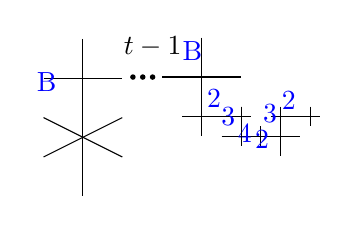
\begin{tikzpicture}[scale=0.5]
     %chain 
  \coordinate (C) at (-1.75, 3.00);
  \coordinate (D) at (-1.25, 3.00);
  \coordinate (A) at (-1.50, 3.00);
  \coordinate (B) at (-1.25, 3.26);
\node[above] at (B) {$t-1$};
  \fill[black] (C) circle (2pt);
  \fill[black] (D) circle (2pt);
  \fill[black] (A) circle (2pt);

%IV
     \coordinate (IVlA) at (-4.02, 2.97);
  \coordinate (IVlB) at (-2.02, 2.97);
  \coordinate (IVlH) at (-3.02, 3.97);
  \coordinate (IVlJ) at (-3.02, -0.03);
  \coordinate (IVlK) at (-4.02, 1.97);
  \coordinate (IVlO) at (-4.02, 0.97);
  \coordinate (IVlP) at (-2.02, 1.97);
  \coordinate (IVlQ) at (-3.94, 2.39);
  \coordinate (IVlN_1) at (-2.02, 0.97);
  \draw (IVlA) -- (IVlB);
  \draw (IVlH) -- (IVlJ);
  \draw (IVlK) -- (IVlN_1);
  \draw (IVlO) -- (IVlP);
  \node[above, text=blue] at (IVlQ) {B};

%III^*
  \coordinate (IIIsrA) at (-1.00, 3.00);
  \coordinate (IIIsrB) at (1.00, 3.00);
  \coordinate (IIIsrC) at (0.00, 4.00);
  \coordinate (IIIsrD) at (0.00, 1.50);
  \coordinate (IIIsrF) at (1.00, 2.00);
  \coordinate (IIIsrE) at (-0.50, 2.00);
  \coordinate (IIIsrH) at (1.00, 2.25);
  \coordinate (IIIsrJ) at (0.50, 1.50);
  \coordinate (IIIsrK) at (2.50, 1.50);
  \coordinate (IIIsrG) at (1.25, 2.00);
  \coordinate (IIIsrN) at (2.00, 2.25);
  \coordinate (IIIsrO) at (2.00, 1.00);
  \coordinate (IIIsrP) at (3.00, 2.00);
  \coordinate (IIIsrQ) at (1.75, 2.00);
  \coordinate (IIIsrA_1) at (-0.24, 3.17);
  \coordinate (IIIsrH_1) at (0.31, 1.97);
  \coordinate (IIIsrJ_1) at (0.67, 1.53);
  \coordinate (IIIsrI_1) at (1.09, 1.10);
  \coordinate (IIIsrP_1) at (2.21, 1.93);
  \coordinate (IIIsrL) at (2.75, 2.25);
  \coordinate (IIIsrM) at (2.75, 1.75);
  \coordinate (IIIsrR) at (1.50, 1.75);
  \coordinate (IIIsrS) at (1.50, 1.25);
  \coordinate (IIIsrI) at (1.00, 1.25);
  \coordinate (IIIsrT) at (1.53, 0.93);
  \coordinate (IIIsrU) at (1.73, 1.60);
\draw (IIIsrA) -- (IIIsrB);
  \draw (IIIsrC) -- (IIIsrD);
  \draw (IIIsrD) -- (IIIsrD);
  \draw (IIIsrF) -- (IIIsrF);
  \draw (IIIsrE) -- (IIIsrG);
  \draw (IIIsrH) -- (IIIsrI);
  \draw (IIIsrJ) -- (IIIsrK);
  \draw (IIIsrE) -- (IIIsrG);
  \draw (IIIsrN) -- (IIIsrO);
  \draw (IIIsrP) -- (IIIsrP);
  \draw (IIIsrP) -- (IIIsrQ);
  \draw (IIIsrP) -- (IIIsrQ);
  \node[above, text=blue] at (IIIsrA_1) {B};
  \node[above, text=blue] at (IIIsrH_1) {$2$};
  \node[above, text=blue] at (IIIsrJ_1) {$3$};
  \node[above, text=blue] at (IIIsrI_1) {$4$};
  \node[above, text=blue] at (IIIsrP_1) {$2$};
  \draw (IIIsrL) -- (IIIsrM);
  \draw (IIIsrR) -- (IIIsrS);
  \draw (IIIsrH) -- (IIIsrI);
  \node[above, text=blue] at (IIIsrT) {$2$};
  \node[above, text=blue] at (IIIsrU) {$3$};

  
\end{tikzpicture}


\end{document}
